\RequirePackage{luatex85}
\documentclass[border={20pt,20pt,20pt,20pt}]{standalone}

\usepackage[dvipsnames]{xcolor}
\usepackage{tikz}
\usetikzlibrary{shapes, patterns, calc}

\begin{document}
	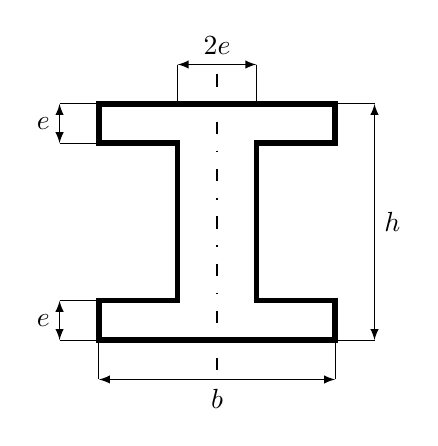
\begin{tikzpicture}[
		arrow/.style={latex-latex},
		scale=0.5
	]
	\draw[line width=2pt] (-3, 3) -- (3, 3) -- (3, 2) -- (1, 2) -- (1, -2) -- (3, -2) -- (3, -3) -- (-3, -3) 
		-- (-3, -2) -- (-1, -2) -- (-1, 2) -- (-3, 2) -- cycle;
	
	
	\draw[arrow] (-1, 4) -- (1, 4) node[above, midway]{$2e$};
	\draw[arrow] (-4, 2) -- (-4, 3) node[midway, left]{$e$};
	\draw[arrow] (-4, -2) -- (-4, -3) node[midway, left]{$e$};
	\draw[arrow] (-3, -4) -- (3, -4) node[midway, below]{$b$};
	\draw[arrow] (4, -3) -- (4, 3) node[midway, right]{$h$};
	
	\draw (-1, 4) -- (-1, 3);
	\draw (1, 4) -- (1, 3);
	
	\draw (-4, 3) -- (-3, 3);
	\draw (-4, 2) -- (-3, 2);
	
	\draw (-4, -3) -- (-3, -3);
	\draw (-4, -2) -- (-3, -2);
	
	\draw (-3, -3) -- (-3, -4);
	\draw (3, -3) -- (3, -4);
	
	\draw (3, 3) -- (4, 3);
	\draw (3, -3) -- (4, -3);
	
	\scalebox{1.5}{
		\draw[loosely dashdotted] (0, 2.5) -- (0, -2.5);
	}
	\end{tikzpicture}
\end{document}